\section{Modelação da base de dados} \label{section: Modelacao}

\subsection{Diagramas, tabelas e modelos}
Com as funcionalidades da aplicação definidas o próximo passo foi modelar a base de dados criando as tabelas e desenhando o diagrama de Entidade-Relacionamento Estendido(EER) através da ferramenta \textit{MySQL Workbench}.

\subsubsection{Tabelas}

Criámos as tabelas tendo em conta as funcionalidades da aplicação:

\begin{itemize}

    \vspace{6pt}
    \item \textbf{user:}
     Dados dos utilizadores registados na aplicação.
    \begin{table}[H]
        \rowcolors{2}{gray!10}{white}
        \centering
        \begin{tabularx}{\linewidth}{XXXXX}
        \toprule
        \textbf{\color{color_scheme}Nome} & \textbf{\color{color_scheme}Tipo} & \textbf{\color{color_scheme}Atributos} & \textbf{\color{color_scheme}Padrão / Expressão}\\
        \midrule
        \texttt{user\_id} & \texttt{INT} & \texttt{PK - NN - AI} &\\
        \texttt{vendor\_id} & \texttt{INT}  & \texttt{FK}  & \texttt{NULL} \\
        \texttt{first\_name} & \texttt{VARCHAR(100)}  & \texttt{NN}  & \\
        \texttt{last\_name} & \texttt{VARCHAR(100)}  & \texttt{NN}  & \\
        \texttt{email} & \texttt{VARCHAR(100)}  & \texttt{NN - UQ}  & \\
        \texttt{deleted} & \texttt{TINYINT}  & \texttt{NN}  & \texttt{0} \\
        \bottomrule
        \end{tabularx}
        \label{table: user}
    \end{table}

    \vspace{3pt}
    \item \textbf{home\_address:}
    Moradas de entrega associadas aos utilizadores. 
    \begin{table}[H]
        \rowcolors{2}{gray!10}{white}
        \centering
        \begin{tabularx}{\linewidth}{XXXXX}
        \toprule
        \textbf{\color{color_scheme}Nome} & \textbf{\color{color_scheme}Tipo} & \textbf{\color{color_scheme}Atributos} & \textbf{\color{color_scheme}Padrão / Expressão}\\
        \midrule
        \texttt{home\_address\_id} & \texttt{INT} & \texttt{PK - NN - AI} &\\
        \texttt{user\_id} & \texttt{INT}  & \texttt{NN - FK}  &  \\
        \texttt{first\_name} & \texttt{VARCHAR(100)}  & \texttt{NN}  & \\
        \texttt{last\_name} & \texttt{VARCHAR(100)}  & \texttt{NN}  & \\
        \texttt{phone\_number} & \texttt{CHAR(9)}  & \texttt{NN - UQ}  & \\
        \texttt{street\_address} & \texttt{VARCHAR(100)}  & \texttt{NN}  & \\
        \texttt{postal\_code} & \texttt{CHAR(8)}  & \texttt{NN}  & \\
        \texttt{city} & \texttt{VARCHAR(100)}  & \texttt{NN}  & \\
        \texttt{comment} & \texttt{MEDIUMTEXT}  &  & \\
        \texttt{deleted} & \texttt{TINYINT}  & \texttt{NN}  & \texttt{0} \\
        \bottomrule
        \end{tabularx}
        \label{table: address_home}
    \end{table}

    \newpage

    \item \textbf{product:}
    Produtos inseridos pelos vendedores. 
    \begin{table}[H]
        \rowcolors{2}{gray!10}{white}
        \centering
        \begin{tabularx}{\linewidth}{XXXXX}
        \toprule
        \textbf{\color{color_scheme}Nome} & \textbf{\color{color_scheme}Tipo} & \textbf{\color{color_scheme}Atributos} & \textbf{\color{color_scheme}Padrão / Expressão}\\
        \midrule
        \texttt{product\_id} & \texttt{INT} & \texttt{PK - NN - AI} &\\
        \texttt{product\_name} & \texttt{VARCHAR(100)}  & \texttt{NN}  & \\
        \texttt{description} & \texttt{MEDIUMTEXT}  & \texttt{NN}  & \\
        \texttt{discount} & \texttt{DOUBLE}  & \texttt{NN - UQ}  & \texttt{0.0}\\
        \texttt{image\_link} & \texttt{VARCHAR(250)}  &  & \\
        \texttt{price} & \texttt{DOUBLE}  & \texttt{NN - UQ}  & \\
        \texttt{stock} & \texttt{INT}  & \texttt{NN - UQ}  & \\
        \texttt{is\_unit} & \texttt{TINYINT}  & \texttt{NN - UQ} & \texttt{0} \\
        \bottomrule
        \end{tabularx}
        \label{table: product}
    \end{table}

    \vspace{3pt}

    \item \textbf{category:}
    Categorias dos produtos. 
    \begin{table}[H]
        \rowcolors{2}{gray!10}{white}
        \centering
        \begin{tabularx}{\linewidth}{XXXXX}
        \toprule
        \textbf{\color{color_scheme}Nome} & \textbf{\color{color_scheme}Tipo} & \textbf{\color{color_scheme}Atributos} & \textbf{\color{color_scheme}Padrão / Expressão}\\
        \midrule
        \texttt{category\_id} & \texttt{INT} & \texttt{PK - NN - AI} &\\
        \texttt{category\_name} & \texttt{VARCHAR(100)}  & \texttt{NN}  & \\
        \bottomrule
        \end{tabularx}
        \label{table: categories}
    \end{table}

    \vspace{3pt}

    \item \textbf{product\_gallery:}
    Galeria de imagens dos produtos. 
    \begin{table}[H]
        \rowcolors{2}{gray!10}{white}
        \centering
        \begin{tabularx}{\linewidth}{XXXXX}
        \toprule
        \textbf{\color{color_scheme}Nome} & \textbf{\color{color_scheme}Tipo} & \textbf{\color{color_scheme}Atributos} & \textbf{\color{color_scheme}Padrão / Expressão}\\
        \midrule
        \texttt{product\_gallery\_id} & \texttt{INT} & \texttt{PK - NN - AI} &\\
        \texttt{product\_id} & \texttt{INT} & \texttt{NN - FK} & \\
        \texttt{image\_link} & \texttt{VARCHAR(250)}  & \texttt{NN} & \\
        \bottomrule
        \end{tabularx}
        \label{table: product_gallery}
    \end{table}

    \vspace{3pt}

    \item \textbf{product\_category:}
    Ligação entre produtos e categorias. 
    \begin{table}[H]
        \rowcolors{2}{gray!10}{white}
        \centering
        \begin{tabularx}{\linewidth}{XXXXX}
        \toprule
        \textbf{\color{color_scheme}Nome} & \textbf{\color{color_scheme}Tipo} & \textbf{\color{color_scheme}Atributos} & \textbf{\color{color_scheme}Padrão / Expressão}\\
        \midrule
        \texttt{product\_id} & \texttt{INT} & \texttt{PK - NN - FK} &\\
        \texttt{category\_id} & \texttt{INT} & \texttt{PK - NN - FK} &\\
        \bottomrule
        \end{tabularx}
        \label{table: product_categories}
    \end{table}
   
    \newpage

    \item \textbf{product\_review:}
    Avaliações dos produtos. 
    \begin{table}[H]
        \rowcolors{2}{gray!10}{white}
        \centering
        \begin{tabularx}{\linewidth}{XXXXX}
        \toprule
        \textbf{\color{color_scheme}Nome} & \textbf{\color{color_scheme}Tipo} & \textbf{\color{color_scheme}Atributos} & \textbf{\color{color_scheme}Padrão / Expressão}\\
        \midrule
        \texttt{product\_review\_id} & \texttt{INT} & \texttt{PK - NN - AI} &\\
        \texttt{user\_id} & \texttt{INT} & \texttt{NN - FK} &\\
        \texttt{product\_id} & \texttt{INT} & \texttt{NN - FK} &\\
        \texttt{rating} & \texttt{INT}  & \texttt{NN}  & \\
        \texttt{created} & \texttt{TIMESTAMP}  &  & \texttt{CURRENT\_TIMESTAMP}\\
        \texttt{comment} & \texttt{MEDIUMTEXT}  & \texttt{NN} & \\
        \bottomrule
        \end{tabularx}
        \label{table: product_reviews}
    \end{table}

    \item \textbf{store:}
    Lojas registadas pelos vendedores. 
    \begin{table}[H]
        \rowcolors{2}{gray!10}{white}
        \centering
        \begin{tabularx}{\linewidth}{XXXXX}
        \toprule
        \textbf{\color{color_scheme}Nome} & \textbf{\color{color_scheme}Tipo} & \textbf{\color{color_scheme}Atributos} & \textbf{\color{color_scheme}Padrão / Expressão}\\
        \midrule
        \texttt{store\_id} & \texttt{INT} & \texttt{PK - NN - AI} &\\
        \texttt{vendor\_id} & \texttt{INT} & \texttt{NN - FK} & \\
        \texttt{store\_name} & \texttt{VARCHAR(100)}  & \texttt{NN - UQ} & \\
        \texttt{store\_phone} & \texttt{VARCHAR(9)}  & \texttt{NN} & \\
        \texttt{store\_email} & \texttt{VARCHAR(100)}  & \texttt{NN - UQ} & \\
        \texttt{description} & \texttt{MEDIUMTEXT}  & \texttt{NN} & \\
        \texttt{profile\_picture} & \texttt{VARCHAR(250)} &  & \\
        \texttt{street\_address} & \texttt{VARCHAR(100)} & \texttt{NN} & \\
        \texttt{city} & \texttt{VARCHAR(100)} & \texttt{NN} & \\
        \texttt{postal\_code} & \texttt{CHAR(8)} & \texttt{NN} & \\
        \texttt{deleted} & \texttt{TINYINT}  & \texttt{NN}  & \texttt{0} \\
        \bottomrule
        \end{tabularx}
        \label{table: store}
    \end{table}

    \item \textbf{store\_review:}
    Avaliações das lojas. 
    \begin{table}[H]
        \rowcolors{2}{gray!10}{white}
        \centering
        \begin{tabularx}{\linewidth}{XXXXX}
        \toprule
        \textbf{\color{color_scheme}Nome} & \textbf{\color{color_scheme}Tipo} & \textbf{\color{color_scheme}Atributos} & \textbf{\color{color_scheme}Padrão / Expressão}\\
        \midrule
        \texttt{store\_review\_id} & \texttt{INT} & \texttt{PK - NN - AI} &\\
        \texttt{user\_id} & \texttt{INT} & \texttt{NN - FK} &\\
        \texttt{store\_id} & \texttt{INT} & \texttt{NN - FK} &\\
        \texttt{rating} & \texttt{INT}  & \texttt{NN}  & \\
        \texttt{created} & \texttt{TIMESTAMP}  &  & \texttt{CURRENT\_TIMESTAMP}\\
        \texttt{comment} & \texttt{MEDIUMTEXT}  & \texttt{NN} & \\
        \bottomrule
        \end{tabularx}
        \label{table: store_reviews}
    \end{table}

    \newpage

    \item \textbf{store\_gallery:}
    Galeria de imagens das lojas. 
    \begin{table}[H]
        \rowcolors{2}{gray!10}{white}
        \centering
        \begin{tabularx}{\linewidth}{XXXXX}
        \toprule
        \textbf{\color{color_scheme}Nome} & \textbf{\color{color_scheme}Tipo} & \textbf{\color{color_scheme}Atributos} & \textbf{\color{color_scheme}Padrão / Expressão}\\
        \midrule
        \texttt{store\_gallery\_id} & \texttt{INT} & \texttt{PK - NN - AI} &\\
        \texttt{store\_id} & \texttt{INT} & \texttt{NN - FK} & \\
        \texttt{image\_link} & \texttt{VARCHAR(250)}  & \texttt{NN} & \\
        \bottomrule
        \end{tabularx}
        \label{table: store_gallery}
    \end{table}

    \item \textbf{vendor:}
    Utilizadores que estão registados como vendedores.
    \begin{table}[H]
        \rowcolors{2}{gray!10}{white}
        \centering
        \begin{tabularx}{\linewidth}{XXXXX}
        \toprule
        \textbf{\color{color_scheme}Nome} & \textbf{\color{color_scheme}Tipo} & \textbf{\color{color_scheme}Atributos} & \textbf{\color{color_scheme}Padrão / Expressão}\\
        \midrule
        \texttt{vendor\_id} & \texttt{INT} & \texttt{PK - NN - AI} &\\
        \texttt{user\_id} & \texttt{INT} & \texttt{NN - FK} & \\
        \texttt{nif} & \texttt{CHAR(9)} & \texttt{NN - UQ} & \\
        \texttt{deleted} & \texttt{TINYINT}  & \texttt{NN}  & \texttt{0} \\
        \bottomrule
        \end{tabularx}
        \label{table: vendor}
    \end{table}

    \item \textbf{order:}
    Encomendas feitas pelos utilizadores. 
    \begin{table}[H]
        \rowcolors{2}{gray!10}{white}
        \centering
        \begin{tabularx}{\linewidth}{XXXXX}
        \toprule
        \textbf{\color{color_scheme}Nome} & \textbf{\color{color_scheme}Tipo} & \textbf{\color{color_scheme}Atributos} & \textbf{\color{color_scheme}Padrão / Expressão}\\
        \midrule
        \texttt{order\_id} & \texttt{INT} & \texttt{PK - NN - AI} &\\
        \texttt{user\_id} & \texttt{INT}  & \texttt{NN - FK}  &  \\
        \texttt{street\_address} & \texttt{VARCHAR(100)}  & \texttt{NN}  & \\
        \texttt{postal\_code} & \texttt{CHAR(8)}  & \texttt{NN}  & \\
        \texttt{city} & \texttt{VARCHAR(100)}  & \texttt{NN}  & \\
        \texttt{created} & \texttt{TIMESTAMP}  &  & \texttt{CURRENT\_TIMESTAMP}\\
        \texttt{comment} & \texttt{MEDIUMTEXT}  &  & \\
        \texttt{status} & \texttt{ENUM()}  & \texttt{NN}  &  \\
        \bottomrule
        \end{tabularx}
        \label{table: order}
    \end{table}

        \item \textbf{order\_product:}
        Produtos que fazem parte das encomendas. 
        \begin{table}[H]
            \rowcolors{2}{gray!10}{white}
            \centering
            \begin{tabularx}{\linewidth}{XXXXX}
            \toprule
            \textbf{\color{color_scheme}Nome} & \textbf{\color{color_scheme}Tipo} & \textbf{\color{color_scheme}Atributos} & \textbf{\color{color_scheme}Padrão / Expressão}\\
            \midrule
            \texttt{order\_product\_id} & \texttt{INT} & \texttt{PK - NN - AI} &\\
            \texttt{order\_id} & \texttt{INT}  & \texttt{NN - FK}  &  \\
            \texttt{product\_id} & \texttt{INT}  & \texttt{NN - FK}  &  \\
            \texttt{price} & \texttt{DOUBLE}  & \texttt{NN}  & \\
            \texttt{discount} & \texttt{DOUBLE}  & \texttt{NN}  & \texttt{0.0}\\
            \bottomrule
            \end{tabularx}
            \label{table: order_product}
        \end{table}

\end{itemize}

\newpage

\subsubsection{Diagrama EER}
Introduzimos as tabelas criadas no \textit{MySQL Workbench} e criámos os relacionamentos entre elas utilizando as chaves estrangeiras:

\vspace{12pt}

\begin{figure}[H]
    \centering
    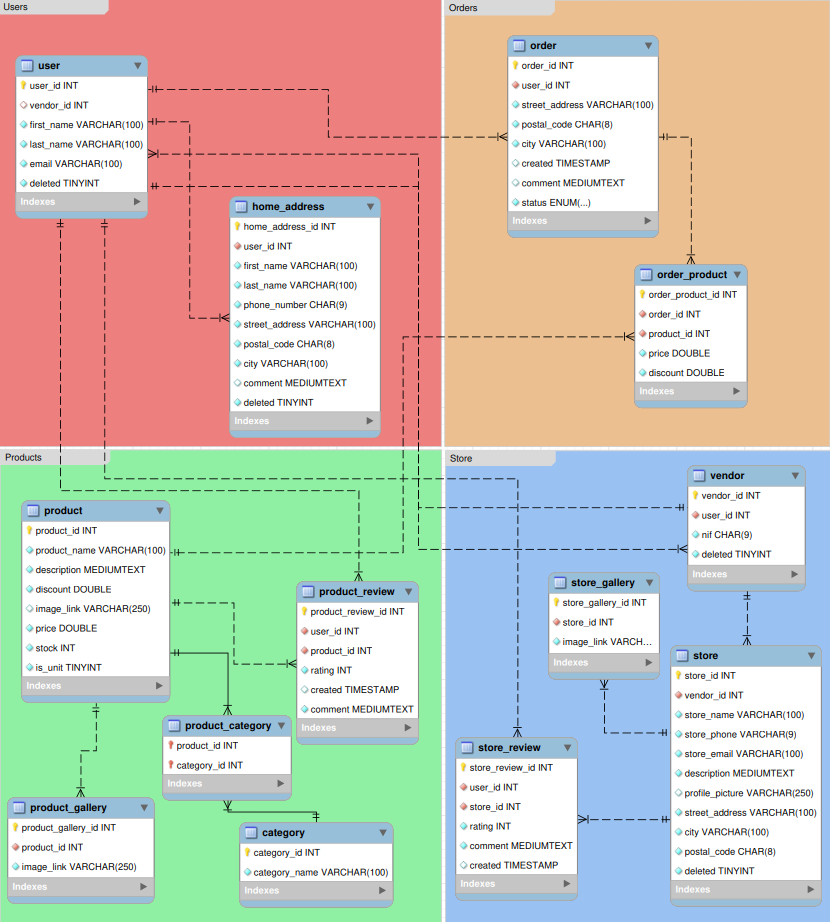
\includegraphics[width=\textwidth]{Figures/0. General/diagram.png}
    \caption{Diagrama EER}
    \label{Diagrama EER}
\end{figure}

\newpage


